%% Submission to Computers and Electronics in Agriculture (Original Research Paper).
%% Format: Elsevier elsarticle, single-column preprint.
\documentclass[preprint,12pt]{elsarticle}

\usepackage[expansion=false]{microtype}
\usepackage{graphicx}
\usepackage{booktabs}
\usepackage{amsmath}
\usepackage{amssymb}
\usepackage{mathtools}
\usepackage{algorithm}
\usepackage{algorithmic}
\usepackage{xcolor}
\usepackage{siunitx}
\usepackage{hyperref}
\usepackage[capitalize,noabbrev]{cleveref}
\usepackage{placeins}
\setlength{\emergencystretch}{3em}

\journal{Computers and Electronics in Agriculture}

\begin{document}

\begin{frontmatter}

\title{An Open-Source Pipeline for Cloud-Native Crop Sequence Boundaries}

\author[a]{Isaac Corley}
\ead{isaac.corley@taylorgeospatial.org}
\affiliation[a]{organization={Taylor Geospatial}}

\begin{abstract}
The USDA Crop Sequence Boundaries (CSB) product partitions the contiguous
United States into field-scale polygons whose attributes encode eight years
of Cropland Data Layer (CDL) classifications. The ArcPy pipeline described by
Hunt et al.~\cite{hunt2024csb} requires an ArcGIS~Pro license and ran for five
days on a 96-core AWS workstation; the authors identify polygon elimination
as its dominant cost. We present an open-source replacement built on
\textsc{rasterio}, \textsc{scikit-image}, \textsc{shapely}, \textsc{DuckDB},
and \textsc{tippecanoe}. We encode each eight-year CDL sequence in a
\texttt{uint64}, avoiding a silent \texttt{int64} overflow in an earlier
base-300 encoding that inflated non-Iowa cropland area by approximately 17\%.
We then reformulate \textsc{Eliminate(LENGTH)} as union-find merge passes over
a connected-component label graph. For validation, an inclusion--exclusion
estimator computes polygon-coverage IoU without dissolving either coverage.
On a single 32-core node, the pipeline produces the 15.30~M-polygon 2018--2025
CONUS dataset in 25.2~min. At the 15 July 2026 lowest regional AWS Spot
snapshot, those stages map to \$0.38 of compute, or \$0.97 including the
optional PMTiles build and parity sweep. Against USDA CSB1825, mean IoU is
0.846 over 16 geographically distributed $5000^2$-pixel tiles (median 0.897;
minimum 0.543). The wall-clock and core-hour ratios relative to the published
USDA runtime are $287\times$ and approximately $860\times$, respectively;
these ratios are not same-hardware benchmarks.
\end{abstract}

\begin{keyword}
crop sequence boundaries \sep cropland data layer \sep open-source GIS \sep
polygon coverage \sep DuckDB \sep agricultural informatics
\end{keyword}

\end{frontmatter}

%-----------------------------------------------------------------------
\section{Introduction}
\label{sec:intro}

The USDA National Agricultural Statistics Service~(NASS) publishes the
Cropland Data Layer~\cite{boryan2011cdl}, an annual 30-meter raster
classification of cultivated crops over the contiguous United States.
For survey design, conservation planning, and agricultural economics
research, NASS additionally distributes the Crop Sequence Boundaries
(CSB) product: a vector layer in which each polygon represents a
per-field unit whose attributes record the CDL class observed in each
of the previous eight years~\cite{hunt2024csb,hunt2024iaos}. CSBs are
used by NASS in the June Area Survey, by the Natural Resources
Conservation Service for crop-rotation summaries, and by the
agricultural economics community as a public proxy for field
boundaries that does not require commercial cadastral data.
\Cref{fig:hero} shows the resulting national coverage and an Iowa comparison
with USDA CSB1825.

The reference implementation of CSB is an ArcPy script using ArcGIS~Pro
geoprocessors. Hunt et al.~\cite{hunt2024csb} report that the 2018--2024 CONUS
build ``took about five days using a 96-core AWS workstation,'' with
``a majority of the processing time \dots\ spent on the
dissolve/elimination step (ArcGIS Pro eliminate function)''. They
further note that ``absent incrementally increasing the selection size,
the tool often fails or takes days.'' The reported compute requirement and
commercial license restrict who can rebuild the national product each year.

We rebuild the pipeline end-to-end in open-source tooling, target a
single-node CPU machine of the type already common in federal HPC
environments, and validate output against the released USDA CSB1825
ground truth. We do not time ArcPy on the same hardware because we do
not have an ArcGIS~Pro license; runtime comparisons therefore use the
published USDA ArcPy runtime reported for the same public reference
workflow~\cite{hunt2024csb,usda_csb_repo}.
The paper makes five contributions:

\begin{itemize}
    \item A \texttt{uint64} bit-packed CDL combine that replaces ArcGIS's
          iterative raster overlay with a single \texttt{numpy.bitwise\_or}
          per year (\cref{sec:method-combine}). We document a base-300
          \texttt{int64} encoding which silently overflowed and inflated
          non-Iowa cropland area by approximately 17\%; the bit-packed form is
          exact.
    \item A raster-side reformulation of \textsc{Eliminate(LENGTH)} as
          connected-component labelling, exact pixel-edge adjacency
          counting, and union-find merging, with a single polygonize call
          at the end (\cref{sec:method-eliminate}). The step runs in
          $0.43\,\text{s}$ on a $2500^2$ Iowa tile; a SedonaDB polygon-side
          baseline crashes at the production $5000^2$ size. A final
          same-combo pass merges class-matched adjacent labels
          (\cref{sec:method-dissolve}).
    \item An exact pairwise inclusion--exclusion estimator for IoU
          between two polygon coverages (\cref{sec:val-method}) that
          parallelises the spatial join in DuckDB and finishes the
          densest parity tile in 25~s, versus $\geq 10$~min for the
          natural \texttt{unary\_union}-then-intersect formulation that
          dispatches single-threaded GEOS.
    \item GeoParquet and PMTiles distributions. GeoParquet replaces the zipped
          ESRI File Geodatabase that USDA currently ships, polygonization
          stays in Apache Arrow throughout the pipeline via the
          \textsc{contourrs} library~\cite{contourrs}, and the national
          coverage can be packaged as one range-addressable PMTiles archive
          (\cref{sec:method-cloud}).
    \item A measured comparison against the USDA reference: 25.2~min wall
          time, \$0.38 of modeled AWS Spot compute at the 15 July 2026
          snapshot, mean IoU 0.846 across 16 diverse tiles, and source code
          available under Apache-2.0 (\cref{sec:results}).
\end{itemize}

\begin{figure}[t]
\centering
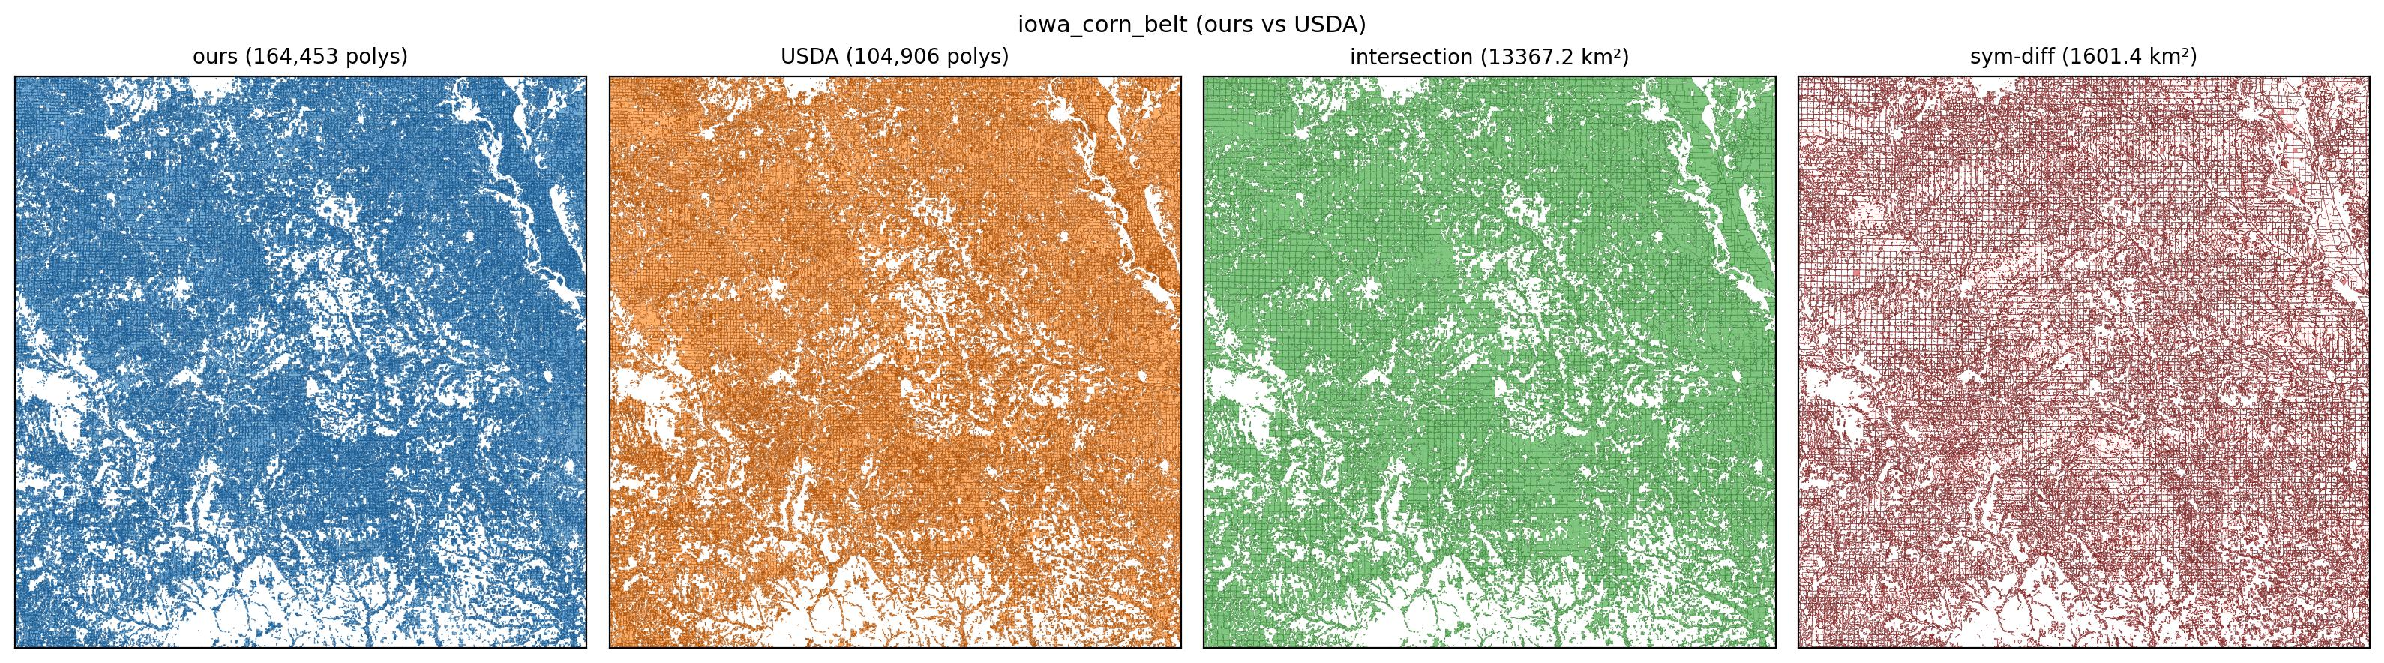
\includegraphics[width=\linewidth]{figures/hero_conus.pdf}
\caption{\textbf{CONUS Crop Sequence Boundaries.} 15.30~M polygons,
2018--2025 CDL combine, generated on a single 32-core node in 25.2~min
from CDL rasters and an Overture-derived road and rail mask. The inset
compares an Iowa tile with USDA CSB1825: shared boundaries are grey,
ours-only boundaries are blue, and USDA-only boundaries are red.}
\label{fig:hero}
\end{figure}

%-----------------------------------------------------------------------
\section{The USDA Reference Implementation}
\label{sec:usda}

The CSB algorithm operates on $N$ annual CDL rasters. The public ArcPy
implementation first uses \texttt{arcpy.gp.Combine\_sa} to enumerate unique
$N$-tuples of CDL classes, then vectorizes the combined raster and attaches
the annual attributes~\cite{hunt2024csb,usda_csb_repo}. Four
\texttt{Eliminate} passes absorb polygons below
$\SI{100}{\meter\squared}$, $\SI{1000}{\meter\squared}$, and twice
$\SI{10000}{\meter\squared}$ into the neighbor with the longest shared
boundary. Next, \texttt{cartography.SimplifyPolygon} applies
\textsc{BEND\_SIMPLIFY} at 60~m while preserving shared-edge topology. A
\textsc{LARGEST\_OVERLAP} spatial join attaches county, agricultural
statistics district (ASD), and state attributes before the output is split
by state.

The dominant cost is step~(iv). Our profiling of an in-house port that
re-implemented elimination as polygon-side cross-joins under
SedonaDB~\cite{yu2019sedona} confirms the diagnosis: at the production
$5000^2$-pixel tile size the WKB blob array exceeds 2~GB and Arrow's
\texttt{int32} offsets overflow, crashing the run. We therefore perform
elimination on raster labels before polygonization.

%-----------------------------------------------------------------------
\section{Method}
\label{sec:method}

\Cref{fig:pipeline} summarises the data flow. We describe each stage
that differs materially from the ArcPy reference.

\begin{figure}[t]
\centering
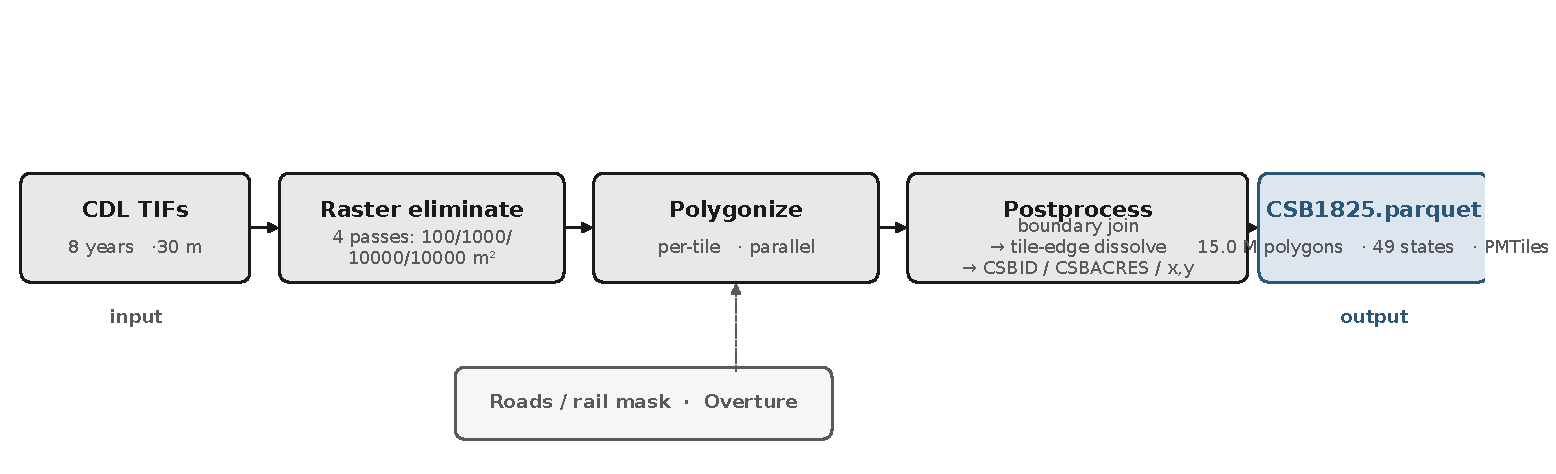
\includegraphics[width=\linewidth]{figures/pipeline.pdf}
\caption{\textbf{Pipeline.} Parallel phase~1 reads each eight-year CDL tile,
packs its classes into \texttt{uint64}, labels connected components, runs four
raster-side elimination passes, and polygonizes once. Streaming phase~2
attaches county, ASD, and state attributes; computes CSBID and CSBACRES; and
partitions the output by state.}
\label{fig:pipeline}
\end{figure}

\subsection{Combine via \texttt{uint64} bit-packing}
\label{sec:method-combine}

The CDL classification scheme uses byte values
$0,\ldots,254$~\cite{boryan2011cdl}; class 254 (BARREN) is the largest
non-sentinel code. With $N=8$ years we therefore have 8~bytes of
information per pixel, which fits exactly in a \texttt{uint64}. We
encode

\[
c(\mathbf{x}) \;=\; \bigvee_{y=1}^{8} \bigl(\,\text{CDL}_y(\mathbf{x}) \ll 8(y-1)\bigr),
\]

implemented as a single \texttt{numpy.bitwise\_or} per year. Downstream stages
use the combined raster as an opaque \texttt{uint64} key for labelling. We
recover each annual attribute as
$\text{CDL}_y = (c \gg 8(y-1)) \,\&\, \mathtt{0xFF}$ during polygonization.
This encoding eliminates the post-hoc
zonal-statistics pass over eight national rasters (approximately 15~GB each)
that the reference pipeline performs through \texttt{JoinField}, which
in our earlier port dominated total wall and triggered
\textsc{exactextract} segfaults on tiles with $>$190k features.

An earlier version used base-$300$ \texttt{int64} encoding,
$c = \sum_y \text{CDL}_y \cdot 300^{y-1}$. Although $300^7 \approx
2.19 \times 10^{17}$ fits in \texttt{int64}, the multiplication by
the year-8 class can reach $254 \cdot 300^7 \approx 5.55 \times 10^{19}$,
which overflows \texttt{int64} silently in NumPy. Iowa did not expose the
overflow because CDL classes 1 (corn) and 5 (soybeans) dominate its pixels and
keep the running sum small. Regions with higher CDL codes had approximately 17\%
excess cropland area. Bit-packing removes this overflow mode.

\subsection{Raster-side \textsc{Eliminate(LENGTH)}}
\label{sec:method-eliminate}

ArcGIS \texttt{Eliminate} in \textsc{LENGTH} mode merges each polygon below an
area threshold into the neighbor with the longest shared boundary. Before
vectorization, pixel-edge counts provide these shared boundary lengths
directly on the label raster.

Let $L \in \mathbb{Z}^{H \times W}$ be the connected-component
labelling of the masked combine raster (\textsc{scikit-image}'s
\texttt{label} with 4-connectivity)~\cite{vanderwalt2014scikit}. Define the
adjacency multiset

\[
A(\ell, \ell') \;=\; \bigl|\{(\mathbf{x}, \mathbf{x}') :
   L(\mathbf{x})=\ell,\, L(\mathbf{x}')=\ell',\, \mathbf{x}'\!-\!\mathbf{x} \in \{e_1, e_2\}\}\bigr|,
\]

the number of horizontal and vertical pixel-edge crossings between
labels $\ell$ and $\ell'$. With pixel pitch $\Delta = 30$~m, the shared
boundary length in metres is $\Delta \cdot A(\ell, \ell')$. We compute
$A$ in a single pass over $L$ as two NumPy slice differences,
$\mathcal{O}(WH)$ time and $\mathcal{O}(|\{\ell\}|)$ memory after a
sparse accumulation.

For each area pass $t \in \{100, 1000, 10000, 10000\}\,\si{\meter\squared}$
(matching the USDA schedule), \cref{alg:eliminate} states the procedure.
After the four passes complete, we polygonize $L$ exactly once.

\begin{algorithm}[t]
\caption{Raster-side \textsc{Eliminate(LENGTH)} pass}
\label{alg:eliminate}
\begin{algorithmic}[1]
\REQUIRE label raster $L$, adjacency $A$, area threshold $t$
\STATE $S_t \gets \{\ell : \text{area}(\ell) < t\}$
\STATE $\text{uf} \gets \text{UnionFind}(\{\ell\})$
\FOR{$\ell \in S_t$ in ascending area order}
    \STATE $\ell^\star \gets \arg\max_{\ell' \notin S_t,\, A(\ell,\ell')>0} A(\ell, \ell')$
    \IF{$\ell^\star$ exists}
        \STATE $\text{uf.union}(\ell, \ell^\star)$
    \ENDIF
\ENDFOR
\STATE $L(\mathbf{x}) \gets \text{uf.find}(L(\mathbf{x}))$ \COMMENT{vectorised}
\STATE recompute $A$, $\text{area}$ on collapsed labels
\end{algorithmic}
\end{algorithm}

The resulting per-tile elimination wall on Iowa is 0.43~s at $2500^2$
and 2.09~s at $5000^2$, against an in-house SedonaDB cross-join baseline
that took 17.6~s at $2500^2$ and crashed at $5000^2$
(\cref{tab:eliminate}).

\begin{table}[t]
\centering
\caption{\textbf{Elimination wall time on one Iowa Q30 tile.} The legacy
implementation uses a SedonaDB polygon-side cross-join; the raster
implementation uses the adjacency graph. End-to-end time includes I/O,
polygonization, and simplification.}
\label{tab:eliminate}
\small
\begin{tabular}{lccc}
\toprule
& $1000^2$ & $2500^2$ & $5000^2$ \\
\midrule
eliminate, legacy   & 1.99 s & 17.58 s & \textsc{crash} \\
eliminate, raster   & 0.07 s & 0.43 s  & 2.09 s \\
end-to-end, legacy  & 2.92 s & 20.25 s & \textsc{crash} \\
end-to-end, raster  & 0.97 s & 4.92 s  & 18.5 s \\
\bottomrule
\end{tabular}
\end{table}

\subsection{Same-combo dissolve}
\label{sec:method-dissolve}

\textsc{Eliminate} merges polygons below the minimum mapping unit (MMU) but
does not merge
above-threshold neighbours that share an identical CDL sequence. After
elimination we observe label pairs $(\ell, \ell')$ with
$\text{area}(\ell), \text{area}(\ell') \geq \text{MMU}$,
$A(\ell, \ell') > 0$, and $c(\ell) = c(\ell')$, where $c$ is the
\texttt{uint64} combine key from \cref{sec:method-combine}. Such pairs
correspond to spatially adjacent fields with identical 8-year crop
histories and are aggregated into single MultiPolygons by the USDA
reference. We add a fifth pass that union-finds all such pairs over
the post-elimination label graph and rewrites $L$ accordingly. On Iowa I15,
the four elimination passes already absorb every class-matched adjacency,
and the additional pass leaves the output unchanged
(\cref{sec:results-ablation}). We retain the pass for tiles where the
longest-shared-edge tiebreak leaves class-matched pairs.

\subsection{Coverage-aware simplification}
\label{sec:method-simplify}

We replace per-polygon Douglas--Peucker simplification with Shapely's
\texttt{coverage\_simplify} at 30~m tolerance and
\texttt{simplify\_boundary=True}~\cite{shapely}. The function applies a
single simplification to each shared edge, preserving consistency between
neighboring polygons. ArcGIS \textsc{BEND\_SIMPLIFY} provides the analogous
coverage-aware operation~\cite{wang1998bend}. Independent per-polygon
simplification instead processes each shared edge twice and can introduce
seams.

\subsection{Postprocessing}
\label{sec:method-postprocess}

Per-tile polygons are written to GeoParquet~1.1 with full PROJJSON CRS
metadata~\cite{geoparquet,kelsey2023geoparquet} and concatenated. The
\textsc{LARGEST\_OVERLAP} spatial join against TIGER/NASS-ASD
boundaries is expressed in DuckDB-spatial as

\begin{verbatim}
SELECT * FROM (
  SELECT a.*, b.STATEFIPS, b.STATEASD, ...,
         ROW_NUMBER() OVER (
           PARTITION BY a.row_id
           ORDER BY ST_Area(
             ST_Intersection(a.geom,b.geom)) DESC
         ) AS rn
  FROM polys a JOIN asd b
       ON ST_Intersects(a.geom,b.geom)
) WHERE rn = 1;
\end{verbatim}

The same query computes CSBID, CSBACRES, INSIDE\_X, and INSIDE\_Y. A
partitioned write keyed by STATEFIPS produces the state GeoParquet files. We
unpack the CDL$_y$ columns from the \texttt{uint64} key carried through
phase~1 instead of recomputing them with zonal statistics.

\subsection{Streaming pipeline}
\label{sec:method-streaming}

A two-phase driver originally synchronized globally between phase~1
(polygonize) and phase~2 (postprocess), leaving cores idle during the join. A
bounded \texttt{multiprocessing.Queue} now connects the phases: each phase~1
worker enqueues completed tile files, and a phase~2 pool processes them as
they arrive. On a 32-core node, this queue removes a 3-min idle period at the
end of phase~1.

\subsection{Cloud-native data products}
\label{sec:method-cloud}

USDA distributes CSB as an approximately 8~GB zipped ESRI File Geodatabase.
Querying a county requires FileGDB support and access to the national archive.
We instead generate three open-format data products.

\paragraph{Polygonization} Phase~1 uses \textsc{contourrs}~\cite{contourrs}, a
Rust raster-polygonization library with Python bindings that emits Arrow
arrays of WKB geometries. Tiles remain in Arrow tables from polygonization to
the GeoParquet write, without intermediate Shapely objects.

\paragraph{GeoParquet distribution} The pipeline writes the national output
as a Hilbert-sorted GeoParquet~1.1 file with explicit
\texttt{xmin/ymin/xmax/ymax} bbox columns per row group
(\cref{sec:val-method}). Consumers can read a county-sized AOI in
sub-second time with DuckDB-spatial without scanning the full 6~GB file.

\paragraph{PMTiles archive} The visualization stage builds one PMTiles
archive~\cite{pmtiles} (2.7~GB for CONUS, zooms 4--12) with
\textsc{tippecanoe} and \textsc{tile-join}~\cite{tippecanoe}. HTTP range
requests allow a
MapLibre GL JS~\cite{maplibre} client to fetch only the tiles in the current
viewport.

%-----------------------------------------------------------------------
\section{Validation Methodology}
\label{sec:val-method}

We compare our polygon coverage $\mathcal{O}$ with USDA coverage
$\mathcal{U}$ inside a test bounding box $B$. Each coverage is
non-overlapping by construction, so each cropland-mask pixel belongs to at
most one polygon. Inclusion--exclusion gives

\begin{align}
A_\mathcal{O}    &= \textstyle\sum_{o\in\mathcal{O}} \text{area}(o \cap B), \\
A_\mathcal{U}    &= \textstyle\sum_{u\in\mathcal{U}} \text{area}(u \cap B), \\
A_\cap           &= \textstyle\sum_{(o,u)} \text{area}(o \cap u \cap B), \\
A_\cup           &= A_\mathcal{O} + A_\mathcal{U} - A_\cap, \\
\text{IoU}(B)    &= A_\cap / A_\cup.
\end{align}

We compute $A_\cap$ with a parallel DuckDB-spatial join, without
\texttt{ST\_Union\_Agg}~\cite{duckdbspatial}. Dissolving each coverage before
intersection dispatches single-threaded GEOS \texttt{unary\_union} over
hundreds of thousands of polygons. The pairwise estimator is exact and
reduces wall time on the densest test tile from $>10$~min to 25~s.

\paragraph{Bounding-box pushdown over GeoParquet}
For per-tile parity, we Hilbert-sort the polygons into 50{,}000-row groups
with explicit \texttt{xmin}, \texttt{ymin}, \texttt{xmax}, and \texttt{ymax}
columns. DuckDB row-group statistics prune $>$99\% of the file for a 150~km
tile query, reducing an Iowa extraction from minutes to 0.6~s. We apply the
same preparation to USDA \texttt{CSB1825.gdb} after conversion to GeoParquet
with GDAL/OGR.

%-----------------------------------------------------------------------
\section{Results}
\label{sec:results}

\subsection{Runtime and cost}
\label{sec:results-runtime}

We measure all stages on a single Taylor Geospatial RAILS \texttt{cpu} partition
node (Intel Xeon Platinum 8468 Sapphire Rapids, 32 physical cores,
256~GB RAM). \Cref{tab:runtime} reports the end-to-end CONUS rebuild.

\begin{table}[t]
\centering
\caption{\textbf{End-to-end CONUS runtime on one 32-core, 256~GB node.}
Polygonization processes 405 tiles and skips 215 tiles without cropland.
Postprocessing writes one national file and 48 state files.}
\label{tab:runtime}
\small
\begin{tabular}{lcc}
\toprule
Stage & Wall & Output \\
\midrule
\texttt{polygonize}  & 13.3 min & 15.30 M polygons \\
\texttt{postprocess} & 11.9 min & national + 48 states \\
\midrule
\textbf{Total}       & \textbf{25.2 min} & USDA-schema parquet \\
\bottomrule
\end{tabular}
\end{table}

\begin{table}[t]
\centering
\small
\caption{\textbf{Single-thread stage runtime on one $5000\times5000$-pixel I15
tile.} Shapely \texttt{coverage\_simplify} accounts for 53.9\% of the
24.87~s total; raster elimination accounts for 8.4\%.}
\label{tab:stage-breakdown}
\begin{tabular}{@{}lrr@{}}
\toprule
Stage & Wall (s) & \% of tile \\
\midrule
\multicolumn{3}{@{}l}{\emph{Load \& key construction}} \\
\quad load\_window (CDL read I/O) & 2.89 & 11.6 \\
\quad combine\_unique (uint64 pack) & 3.45 & 13.9 \\
\midrule
\multicolumn{3}{@{}l}{\emph{Raster pipeline}} \\
\quad mask & 0.07 & 0.3 \\
\quad label\_cc (4-conn CC) & 0.56 & 2.3 \\
\quad label\_to\_combo & 0.18 & 0.7 \\
\quad numpy\_filter & 0.32 & 1.3 \\
\quad eliminate\_raster (4-pass) & 2.09 & 8.4 \\
\midrule
\multicolumn{3}{@{}l}{\emph{Vector emit}} \\
\quad polygonize\_once & 1.20 & 4.8 \\
\quad eff\_lookup & 0.69 & 2.8 \\
\quad simplify\_shapely & 13.41 & 53.9 \\
\midrule
\textbf{Total} & \textbf{24.87} & \textbf{100.0} \\
\bottomrule
\end{tabular}
\end{table}

\begin{figure}[t]
\centering
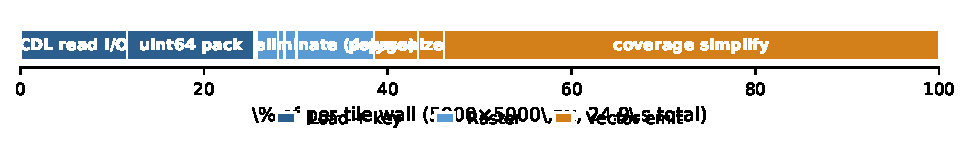
\includegraphics[width=\linewidth]{figures/stage_breakdown.pdf}
\caption{\textbf{Stage runtime on a $5000^2$ Iowa tile.} Coverage
simplification accounts for 53.9\% of wall time, compared with 8.4\% for the
four raster-elimination passes.}
\label{fig:stage-breakdown}
\end{figure}

The USDA ArcPy workflow described by Hunt et
al.~\cite{hunt2024csb,usda_csb_repo} reports 5 days on a 96-core AWS
workstation, or 11{,}520 core-hours. Our 25-min run on 32 cores uses 13.4
core-hours. Hunt et al.\ do not report the EC2 instance, operating system,
purchase model, or AWS bill. For an illustrative current public-list estimate,
a 96-vCPU \texttt{c6i.24xlarge} running license-included Windows costs
\$8.496/hr on demand, or \$1{,}020 for 120~hr. Our 25-min run maps to
\$1.35 on a Linux \texttt{m7i.16xlarge} on demand or \$0.38 at the 15 July
2026 lowest regional Spot snapshot~\cite{aws_ec2_pricing,aws_spot_pricing}.
Including the
optional PMTiles and parity stages raises the Spot estimate to \$0.97. These
are pricing models, not measured cloud bills. ArcGIS \texttt{Eliminate}
requires an Advanced license~\cite{esri_eliminate}; effective government and
enterprise pricing varies.

\begin{table}[t]
\centering
\caption{\textbf{Published USDA runtime and measured open-source runtime.}
The USDA wall time comes from Hunt et al.~\cite{hunt2024csb}. Cost rows are
illustrative current public-list
equivalents~\cite{aws_ec2_pricing,aws_spot_pricing}, not
measured bills. Hardware, operating systems, and pricing modes differ.}
\label{tab:cost}
\small
\begin{tabular}{lcc}
\toprule
              & USDA (Hunt et al.\ 2024) & This work \\
\midrule
Wall          & 120 hr                   & 0.42 hr \\
Cores         & 96 (AWS)                 & 32 \\
Core-hours    & 11{,}520                 & 13.4 \\
EC2 on-demand & \$1{,}020 (Windows)       & \$1.35 (Linux) \\
EC2 spot      & \$579 (Windows)           & \$0.38 (Linux) \\
Required GIS tier & ArcGIS Pro Advanced   & None \\
Output        & $<$20 M polys            & 15.30 M polys \\
Wall speedup  & ---                      & $\mathbf{287\times}$ \\
Core-hour ratio & ---                    & $\mathbf{860\times}$ \\
\bottomrule
\end{tabular}
\end{table}

\paragraph{Scope of the runtime comparison}
We cannot run the ArcPy workflow on the same hardware because our environment
does not have an ArcGIS~Pro license. The $287\times$ wall-clock and
$860\times$ core-hour ratios therefore compare our measurement with the
published USDA runtime; they do not isolate the effects of hardware,
software, or implementation. The controlled comparison in this paper is the
Iowa tile ablation in \cref{tab:eliminate}: raster elimination takes
0.43~s, compared with 17.58~s for our SedonaDB polygon-side implementation on
the same $2500^2$ tile. Our stage profile further shows that coverage
simplification, not elimination, is now the largest measured cost
(\cref{tab:stage-breakdown}).

\subsection{Parity vs.\ USDA CSB1825}
\label{sec:results-parity}

We evaluate parity on 16 $5000^2$-pixel CONUS tiles spanning corn-belt,
cotton, peanut, wheat, sugarcane, mixed-crop, and irrigated-arid regions.
\Cref{tab:parity-summary} summarizes per-tile IoU and acreage parity, and
\cref{tab:parity-detail} reports six regional results.

\begin{table}[t]
\centering
\caption{\textbf{Parity distribution, 16 tiles vs.\ USDA CSB1825.}
IoU computed via the inclusion--exclusion estimator
(\cref{sec:val-method}). Polygon ratio is ours/USDA.}
\label{tab:parity-summary}
\small
\begin{tabular}{lcccc}
\toprule
                & mean & median & min & max \\
\midrule
IoU             & 0.846 & \textbf{0.897} & 0.543 & 0.938 \\
acres ratio     & 0.94  & 0.97           & 0.70  & 1.01 \\
poly ratio      & 1.03  & 0.92           & 0.49  & 1.59 \\
\bottomrule
\end{tabular}
\vspace{0.4em}\\
At full CONUS extent the same metric yields IoU \textbf{0.850}
($n_\text{ours}{=}15.30\,\text{M}$, $n_\text{usda}{=}15.97\,\text{M}$,
acres ratio 0.946, poly ratio 0.958).
\end{table}

\begin{table}[t]
\centering
\caption{\textbf{Parity for six regional tiles.} Each tile covers
$5000^2$ pixels ($150\,\text{km} \times 150\,\text{km}$) and is evaluated
against \texttt{CSB1825.gdb}. Acreage uses the USDA units.}
\label{tab:parity-detail}
\footnotesize
\setlength{\tabcolsep}{4pt}
\begin{tabular}{lcccccc}
\toprule
Region & $n_\text{ours}$ & $n_\text{usda}$ & poly ratio & acres ours & acres USDA & IoU \\
\midrule
Iowa corn belt (I15)        & 166{,}471 & 104{,}906 & 1.59 & 3{,}469{,}259 & 3{,}486{,}519 & 0.913 \\
Texas Panhandle (N11)       &  72{,}222 &  95{,}662 & 0.75 & 2{,}178{,}676 & 2{,}210{,}378 & 0.914 \\
Central Valley CA (K2)      &  11{,}689 &  11{,}256 & 1.04 &   233{,}980   &   248{,}616   & 0.771 \\
Mississippi Delta (N17)     &   6{,}291 &   8{,}640 & 0.73 &   147{,}033   &   160{,}003   & 0.843 \\
Palouse wheat (C3)          &  53{,}120 &  61{,}122 & 0.87 & 2{,}006{,}910 & 2{,}013{,}339 & 0.909 \\
Wisconsin mixed (F17)       & 141{,}932 & 118{,}292 & 1.20 & 3{,}252{,}117 & 3{,}386{,}171 & 0.909 \\
\bottomrule
\end{tabular}
\end{table}

\begin{figure}[t]
\centering
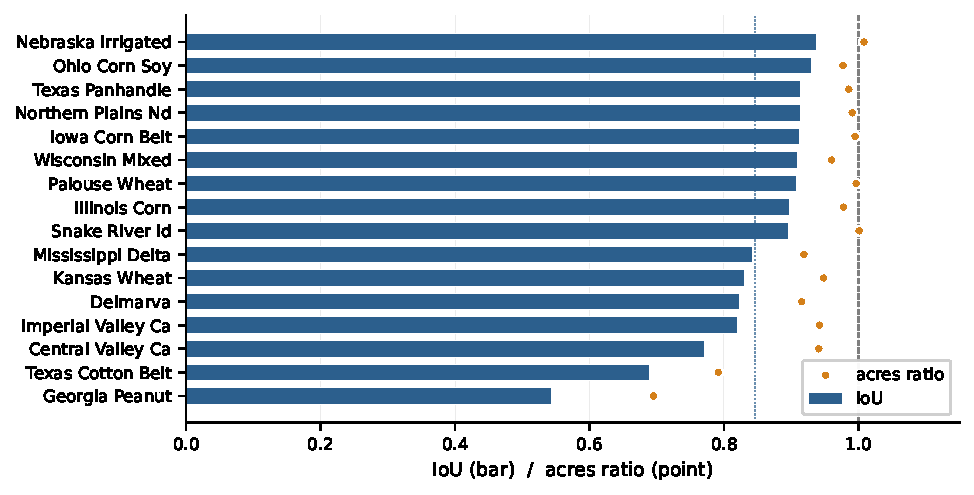
\includegraphics[width=\linewidth]{figures/per_tile_iou.pdf}
\caption{\textbf{Parity over 16 CONUS tiles, sorted by IoU.} Bars show IoU,
and circles show the ours-to-USDA acreage ratio. The dashed line marks equal
acreage; the dotted line marks mean IoU.}
\label{fig:per-tile-iou}
\end{figure}

Nine of the sixteen tiles clear $\text{IoU} \geq 0.89$. The three
lowest-IoU tiles are GA peanut (0.543), TX cotton (0.690), and CA
Central Valley (0.771). All three contain less cropland than the high-IoU
tiles, so a fixed area of disagreement produces a larger IoU change. These
regions also contain many small fields for which the 30~m raster grid,
cropland-mask threshold, and simplification tolerance affect the resulting
boundaries. A one-pixel change along a field edge can split a polygon that
USDA retains as one unit, or conversely merge two units. Adopting USDA's road
and rail
mask via Overture Maps~\cite{overture} (already integrated in our
production runs through \texttt{csb roads-prep} and the
\texttt{--roads-mask} flag) closes a portion of the gap on
mid-density tiles but does not raise the three lowest tile scores. Their
visual differences are concentrated along field boundaries rather than in
large connected regions.

\begin{figure}[t]
\centering
\includegraphics[width=\linewidth]{figures/bottom3_montage.pdf}
\caption{\textbf{Differences for the three lowest-IoU tiles.} Agreement is
grey, ours-only coverage is blue, and USDA-only coverage is red. Most
differences follow field edges rather than large connected regions.}
\label{fig:bottom3-montage}
\end{figure}

\subsection{Per-class agreement vs.\ USDA CSB1825}
\label{sec:results-per-class}

Beyond polygon-coverage IoU, we evaluate per-class agreement on the
2024 CDL labels carried by each polygon. \Cref{tab:per-class} reports,
for the 15 largest CDL classes by USDA acreage, the share of USDA
acreage our pipeline labels with the same code (\emph{Agree}) and the
same metric restricted to USDA pixels retained by our 2-year cropland
mask (\emph{W-mask}), plus the leading crop-vs-crop confusion.

\begin{table}[t]
\centering
\caption{\textbf{Per-class agreement with USDA CSB1825 for 2024.} The table
reports the 15 largest CDL classes by USDA acreage.
\emph{Agree} is the share of USDA acreage for the class that our
pipeline labels with the same CDL code; \emph{W-mask} restricts the
denominator to USDA pixels retained by our 2-year cropland mask.
\emph{Top off-diag.} reports the largest crop-vs-crop confusion.}
\label{tab:per-class}
\small
\setlength{\tabcolsep}{4pt}
\begin{tabular}{@{}rlrrrl@{}}
\toprule
Code & Class & USDA Mac & Agree & W-mask & Top off-diag. \\
\midrule
  1 & Corn                      & 88.39 & 74.5\% & 89.6\% & Soy 6.5\%        \\
  5 & Soybeans                  & 82.14 & 75.4\% & 90.1\% & Corn 6.4\%       \\
 24 & Winter Wheat              & 23.05 & 70.7\% & 89.5\% & Fallow 2.3\%     \\
  2 & Cotton                    & 11.12 & 68.0\% & 86.9\% & Soy 5.2\%        \\
 23 & Spring Wheat              & 10.91 & 69.9\% & 86.1\% & Soy 2.2\%        \\
 61 & Fallow/Idle Cropland      & 10.58 & 68.4\% & 85.5\% & Win.\ Wheat 4.8\%\\
 36 & Alfalfa                   & 10.18 & 56.7\% & 84.1\% & Corn 4.5\%       \\
  4 & Sorghum                   &  6.21 & 67.9\% & 83.6\% & Corn 4.5\%       \\
 26 & Dbl Crop W.Wht/Soy        &  4.02 & 65.0\% & 82.8\% & Soy 8.6\%        \\
  3 & Rice                      &  2.87 & 66.1\% & 78.7\% & Soy 14.9\%       \\
 31 & Canola                    &  2.62 & 68.5\% & 82.8\% & Sp.\ Wheat 5.4\% \\
 21 & Barley                    &  1.83 & 57.2\% & 75.4\% & Sp.\ Wheat 8.2\% \\
 75 & Almonds                   &  1.70 & 69.8\% & 86.0\% & Grapes 3.8\%     \\
 37 & Other Hay/Non-Alfalfa     &  1.70 & 49.5\% & 79.6\% & Alfalfa 8.5\%    \\
 10 & Peanuts                   &  1.64 & 44.3\% & 59.6\% & Cotton 30.9\%    \\
\bottomrule
\end{tabular}
\end{table}

\begin{figure}[t]
\centering
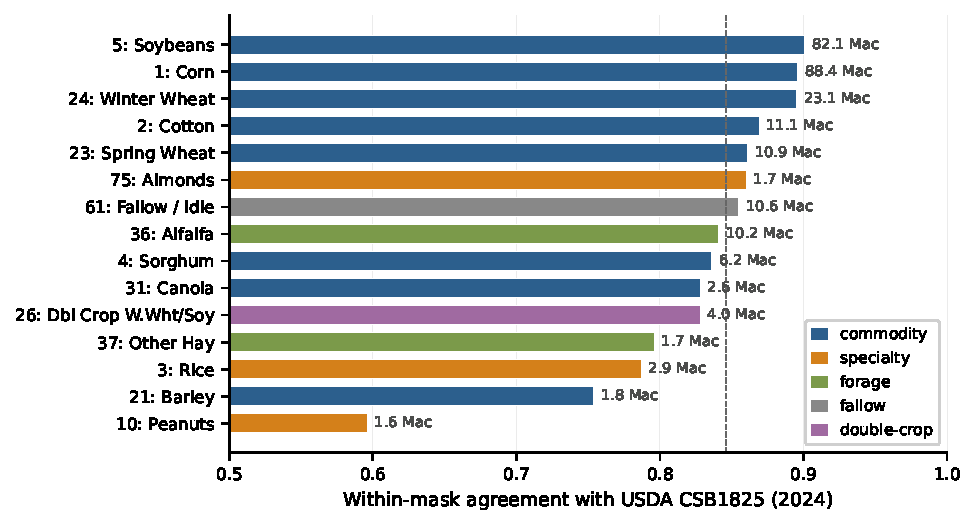
\includegraphics[width=\linewidth]{figures/per_class.pdf}
\caption{\textbf{Within-mask agreement for the 15 largest CDL classes.}
Bars are grouped by crop family; labels report USDA acreage in million acres
(Mac). The dashed line shows the 84.6\% mean polygon-coverage IoU for
orientation, but the two metrics have different denominators.}
\label{fig:per-class}
\end{figure}

Per-class agreement is highest on the major commodity rotations. Within
USDA pixels retained by our 2-year cropland mask, corn (89.6\%), soybeans
(90.1\%), winter wheat (89.5\%), and cotton (86.9\%) have the highest
agreement. The leading confusion for corn and soybeans is a corn--soybean
swap (approximately 6\%). Divergence concentrates in three families: hay and forage
classes (Alfalfa,
Other Hay) where the mode-of-modes label flips between neighbouring
years; small-grain rotations (Barley, Spring Wheat) that inter-confuse
at 8--15\%; and specialty/double-crop classes (Peanuts, Rice, Dbl-Crop
WinWht/Soy) where field counts are low. Roughly 17--22\% of USDA
acreage for every class is attributed to ``no-class'' in our output,
reflecting the 2-year crop-frequency threshold dropping single-year
cropped pixels and simplification eroding sub-acre fields.

\subsection{Simplification and dissolve ablation}
\label{sec:results-ablation}

We re-ran phase~1 on tile~I15 (Iowa corn belt, $5000^2$~px) with the
\textsc{coverage\_simplify} tolerance varied across $\{30, 60, 120\}\,
\text{m}$ and with the same-combo dissolve pass disabled, holding all
other settings fixed. \Cref{tab:ablation} reports the result.

\begin{table}[t]
\centering
\caption{\textbf{Ablation on the $5000^2$-pixel Iowa I15 tile.} The table
reports polygon count, ratios relative to USDA, and IoU against
\texttt{CSB1825.gdb}. These provisional values come from a separate I15 run
and require regeneration before submission.}
\label{tab:ablation}
\small
\begin{tabular}{lcccc}
\toprule
variant                       & $n_\text{ours}$ & $n/n_\text{USDA}$ & acres ratio & IoU \\
\midrule
default (s=30, dissolve)      & 178{,}834 & 1.70 & 1.002 & \textbf{0.905} \\
simplify $60$~m               & 175{,}121 & 1.67 & 0.998 & 0.896 \\
simplify $120$~m              & 159{,}969 & 1.52 & 0.963 & 0.866 \\
no same-combo dissolve        & 178{,}834 & 1.70 & 1.002 & \textbf{0.905} \\
\bottomrule
\end{tabular}
\end{table}

In this tile, tightening the simplification tolerance from 120~m to 30~m
raises IoU by 4 points and brings
the acreage ratio from $0.96$ to $1.00$ at the cost of approximately 12\% more
polygons. USDA's published \textsc{BEND\_SIMPLIFY} runs at 60~m; we set
our default to 30~m (one CDL pixel) because the IoU gain is consistent
across the 16-tile parity sweep. On I15, this choice adds approximately 12\% more
polygons than 120~m simplification. The same-combo dissolve produces
\emph{bit-identical} output on this
tile because the four elimination passes already absorb every class-matched
adjacency. We retain the pass for tiles where the longest-shared-edge
tiebreak leaves class-matched pairs, but this ablation provides evidence only
for Iowa I15.

\begin{figure}[t]
\centering
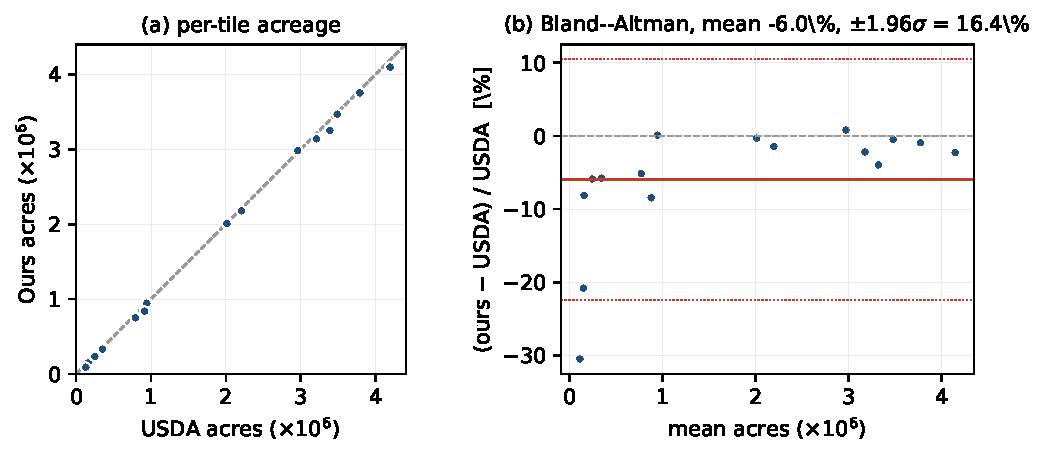
\includegraphics[width=\linewidth]{figures/acres_scatter.pdf}
\caption{\textbf{Acreage parity over 16 CONUS tiles.} Left: ours versus USDA
on a $1\!:\!1$ axis. Right: percent difference versus mean acreage. The mean
offset is $-6.0\%$, the median is $-3.1\%$, and the $\pm1.96\sigma$ interval
is $\pm16\%$.}
\label{fig:acres-scatter}
\end{figure}

\FloatBarrier

%-----------------------------------------------------------------------
\section{Related Work}
\label{sec:related}

\paragraph{The Cropland Data Layer and CSB lineage}
The Cropland Data Layer~\cite{boryan2011cdl} is an established input for
U.S.\ crop mapping. Recent work produces in-season CDL-like maps from
historical trusted-pixel samples and multi-source Sentinel-2 and Landsat
imagery~\cite{li2024automatedcdl,zhang2022inseason}. CSB aggregates these
per-pixel classes into multi-year field-level
polygons~\cite{hunt2024csb,hunt2024iaos}. The NRCS Conservation Effects
Assessment
Project uses CSB to validate rotation imputations from the Agricultural
Policy Environmental eXtender model~\cite{nrcs_ccr_328}.
Bribiesca-Rodriguez et al.~\cite{rodriguezgarcia2025csbeval} evaluate CSB
boundaries for Endangered Species Act overlap analysis in California. They
report acreage overestimation for almonds, grapes, and cotton, along with an
excess field count. These findings motivate quantitative comparison with the
USDA reference rather than visual comparison alone.

\paragraph{Parallel polygon coverage and raster-to-vector at scale}
A line of distributed-systems work addresses large-scale geospatial
processing on commodity clusters. GeoSpark and its successor Apache
Sedona~\cite{yu2019sedona} extend Spark with spatial partitioners,
indices, and join operators; GeoTrellis~\cite{geotrellis} provides a
parallel raster engine on the JVM; and RasterFrames~\cite{rasterframes}
brings raster tiles into Spark DataFrames. None of these target the
specific raster-to-vector elimination workload in CSB. In our Sedona
polygon-side implementation (\cref{sec:usda}), Arrow's \texttt{int32} WKB
offsets overflow below the $5000^2$-pixel production tile size. GDAL
\texttt{Polygonize}~\cite{gdal} provides a pixel-edge walking algorithm; we
use \textsc{contourrs}~\cite{contourrs} because it emits Arrow arrays.

\paragraph{Polygon-coverage simplification}
Per-polygon Douglas--Peucker simplification produces seam artefacts when
applied independently to neighbours that share a boundary, motivating
coverage-aware variants. ArcGIS's \textsc{BEND\_SIMPLIFY} option
implements the bend-based generalisation of Wang and
M\"uller~\cite{wang1998bend}, which detects and smooths shape-bearing
bends while topologically respecting shared edges. The same property
is now available in pure open source through Shapely~2.x's
\texttt{coverage\_simplify}~\cite{shapely,gillies2024shapely2}, which
exposes JTS/GEOS coverage simplification as a vectorised NumPy ufunc.
Because every shared edge is simplified once rather than twice, the
function preserves topological consistency across a non-overlapping
polygon coverage, an essential property for downstream join and
acreage-summation workflows.

\paragraph{Open-source replacements of commercial GIS}
QGIS~\cite{qgis2025patterns} provides open-source desktop GIS and is used by
federal, municipal, and academic organizations.
PostGIS~\cite{obe2021postgis} provides an open-source spatial database, while
GeoPandas~\cite{jordahl2020geopandas} adds spatial types to the pandas and
Arrow ecosystem. DuckDB-spatial~\cite{duckdbspatial} combines DuckDB's
columnar runtime~\cite{raasveldt2019duckdb} with GEOS predicates and GDAL I/O.
Our pipeline uses these components in place of the ArcPy and ArcGIS~Pro stack
described by Hunt et al.~\cite{hunt2024csb}.

\paragraph{Cloud-native geospatial formats}
Several geospatial formats support HTTP range access: Cloud-Optimized
GeoTIFF for rasters~\cite{ogc_cog}, GeoParquet for vector tables with
columnar pruning~\cite{geoparquet,kelsey2023geoparquet}, FlatGeobuf for
streaming feature reads~\cite{flatgeobuf}, STAC for asset
discovery~\cite{stacspec}, and PMTiles for single-archive vector and
raster tilesets~\cite{pmtiles}. Our CSB outputs use GeoParquet for
analytical access and PMTiles for map display. Recent work on field-level
boundary extraction from satellite imagery---ResUNet-style segmentation
in heterogeneous landscapes~\cite{waldner2020deepedge} and transfer
learning into smallholder regimes~\cite{wang2022smallholder}---is
complementary. Those methods infer field geometry from imagery, whereas CSB
aggregates an existing per-pixel classification into polygons with
multi-year crop-history attributes.

%-----------------------------------------------------------------------
\section{Limitations}
\label{sec:limits}

\paragraph{Road and rail mask source} USDA's CSB pipeline rebuilds
its transportation mask each year from a Google Earth Engine pass over
proprietary basemap data. We instead pre-rasterise the open Overture
Maps transportation theme~\cite{overture} (\texttt{csb roads-prep}) and
apply the buffered raster as a mask to the cropland layer prior to
connected-components labelling. The two masks differ in temporal
currency (Overture is community-edited and updated more frequently)
and in coverage of unpaved farm tracks; quantifying their parity is
left to future work.

\paragraph{Eight-year horizon} The \texttt{uint64} bit-packing fits exactly
$8 \cdot 8 = 64$~bits. Longer horizons require multiple \texttt{uint64}
words or an indexed lookup table. We have not implemented either approach.

\paragraph{Tile-edge reconciliation} Postprocessing unions touching polygons
on opposite tile edges when their full CDL sequence matches. Small geometric
gaps or classification disagreements prevent a merge, so some cross-tile
fields can remain split relative to USDA.

\paragraph{CONUS scope} The pipeline does not currently include
Alaska or Hawaii, matching USDA's scope.

%-----------------------------------------------------------------------
\section{Reproducibility}
\label{sec:reproducibility}

The source code is available under the Apache-2.0 license in the
\href{https://github.com/isaaccorley/crop-sequence-boundaries-v2}{project
repository}. The project has not published a Python package release. After
local installation, a full CONUS run uses three
commands: \texttt{csb download 2018 2025}, \texttt{csb build-boundaries},
and \texttt{csb run-all 2018 2025}. SLURM batch scripts for a 96-core
HPC node and a 32-core spot instance are included under
\texttt{examples/cluster/}. A public 2.7~GB
\href{https://source.coop/ftw/usda-csb}{2025 USDA CSB PMTiles archive} is
available, but no versioned release of the 15.30~M-polygon GeoParquet exists
yet. The parity and per-class evaluations therefore require locally generated
output and the USDA CSB1825 reference.
All experiments in this paper used Python~3.12,
\textsc{rasterio}~1.4~\cite{rasterio}, \textsc{shapely}~2.1,
\textsc{DuckDB}~1.2 with
the spatial extension, \textsc{contourrs}~0.7, and \textsc{tippecanoe}~2.61.

%-----------------------------------------------------------------------
\section{Conclusion}

We rebuilt the USDA Crop Sequence Boundaries pipeline with open-source
software. Relative to the published USDA ArcPy runtime envelope, the measured
wall-clock and core-hour ratios are $287\times$ and $860\times$; this is not a
same-hardware comparison. Mean IoU is 0.846 across 16 CONUS tiles. Key
implementation changes include
\texttt{uint64} bit-packing of the multi-year combine and a raster-side
reformulation of \textsc{Eliminate(LENGTH)} as a label-graph union-find,
which addresses the elimination bottleneck identified by
Hunt et al.~\cite{hunt2024csb}. The pipeline runs on a single 32-core node at
\$0.38 of modeled AWS Spot compute for the measured generation stages,
requires no commercial GIS license, and produces outputs with USDA-identical
schema. Source code is available in the project repository. The generated
CONUS dataset has not received a versioned release; the 2025 USDA CSB PMTiles
archive is public.

\section*{Data and Code Availability}

Source code is available under the Apache-2.0 license in the
\href{https://github.com/isaaccorley/crop-sequence-boundaries-v2}{project
repository}. The preview PMTiles archive is public on
\href{https://source.coop/ftw/usda-csb}{Source Cooperative}; the generated
GeoParquet has not received a versioned release. The repository includes the
parity and per-class evaluation code.

\section*{Declaration of Competing Interest}

The author declares no competing financial interests or personal
relationships that could have appeared to influence the work reported in
this paper.

\section*{Funding}

This research did not receive any specific grant from funding agencies in
the public, commercial, or not-for-profit sectors.

\section*{Declaration of Generative AI and AI-Assisted Technologies in the Manuscript Preparation Process}

During preparation of this work the author used OpenAI Codex to assist
with proofreading, LaTeX editing, and consistency checks. The author
reviewed and edited the content as needed and takes full responsibility
for the content of the published article.

\bibliographystyle{elsarticle-num}
\bibliography{csb}

\end{document}
